\documentclass[tikz,border=4pt]{standalone}
% Shared style for every figure and for the deck: one accent, one
% highlight, thin lines, rounded nodes, nothing decorative.
\usepackage[T1]{fontenc}
\usepackage{lmodern}
\renewcommand{\familydefault}{\sfdefault}
\usepackage{tikz}
\usetikzlibrary{arrows.meta,positioning,calc,shapes.misc,fit,backgrounds,decorations.pathreplacing}
\definecolor{ink}{RGB}{40,40,40}
\definecolor{soft}{RGB}{150,150,150}
\definecolor{faint}{RGB}{225,225,225}
\definecolor{accent}{RGB}{0,95,115}
\definecolor{accentlight}{RGB}{214,232,236}
\definecolor{warn}{RGB}{196,84,40}
\definecolor{warnlight}{RGB}{247,226,216}
\tikzset{
  every picture/.style={color=ink, line width=0.5pt, font=\small},
  node distance=12mm and 18mm,
  box/.style={draw=ink, rounded corners=2pt, fill=white, inner sep=5pt, minimum height=7mm, align=center},
  maker/.style={box, minimum width=18mm},
  cat/.style={box, inner sep=3.5pt, minimum height=6mm},
  root/.style={box, fill=accentlight, draw=accent},
  bad/.style={box, fill=warnlight, draw=warn},
  ghost/.style={box, draw=soft, text=soft, dashed},
  flow/.style={-{Stealth[length=4pt,width=3.5pt]}, line width=0.5pt},
  sub/.style={-{Stealth[length=4pt,width=3.5pt]}, line width=0.5pt, color=soft},
  strong/.style={flow, color=accent, line width=0.8pt},
  wrong/.style={flow, color=warn},
  lbl/.style={font=\footnotesize, text=ink, inner sep=1.5pt, fill=white},
  note/.style={font=\footnotesize, text=soft, align=center},
  rate/.style={font=\footnotesize, text=accent, inner sep=1pt, fill=white},
}

\usepackage{amsmath}
\usepackage{pgfplots}
\pgfplotsset{compat=1.17}

\begin{document}
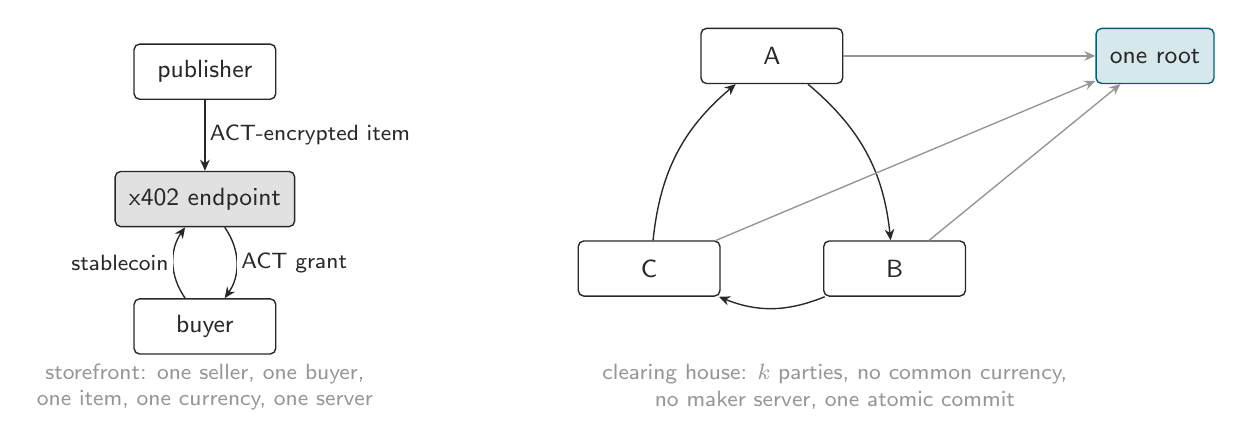
\begin{tikzpicture}
  \begin{scope}
    \node[maker] (pub) {publisher};
    \node[box, below=9mm of pub, fill=faint] (srv) {x402 endpoint};
    \node[maker, below=9mm of srv] (buy) {buyer};
    \draw[flow] (pub) -- node[lbl, right] {ACT-encrypted item} (srv);
    \draw[flow] (buy) to[bend left=35] node[lbl, left] {stablecoin} (srv);
    \draw[flow] (srv) to[bend left=35] node[lbl, right] {ACT grant} (buy);
    \node[note] at (0,-40mm) {storefront: one seller, one buyer,\\ one item, one currency, one server};
  \end{scope}
  \begin{scope}[xshift=72mm, yshift=-16mm]
    \node[maker] (A) at (90:18mm) {A};
    \node[maker] (B) at (-30:18mm) {B};
    \node[maker] (C) at (210:18mm) {C};
    \draw[flow] (A) to[bend left=22] (B); \draw[flow] (B) to[bend left=22] (C); \draw[flow] (C) to[bend left=22] (A);
    \node[root, right=32mm of A] (R) {one root};
    \draw[sub] (A) -- (R); \draw[sub] (B) -- (R); \draw[sub] (C) -- (R);
    \node[note] at (8mm,-24mm) {clearing house: $k$ parties, no common currency,\\ no maker server, one atomic commit};
  \end{scope}
\end{tikzpicture}
\end{document}
